\section{6-DOF model of a Rigid Body}
% =========================================
% =========================================


\begin{frame}{6-DOF model of a Rigid Body}
	\framesubtitle{Goal} 
	\begin{block}{Final goal}
		To find the equations that describe the behavior of the system
		\begin{align}
			M_{RB}\dot{\nu} + C_{RB}\nu = \tau_{RB}
		\end{align}
		in addition, as discussed above, 
		\begin{align}
			\dot{\eta} = J_{\Theta}(\eta)\nu
		\end{align}
	\end{block}
	\begin{itemize}
		\item Newton-Euler equations of motion about CG (Center gravity)
		\item Newton-Euler equations of motion about CO
	\end{itemize}
\end{frame}



% =========================================
% =========================================


\begin{frame}{6-DOF model of a Rigid Body}
	\framesubtitle{Fundamental}
	
	\begin{block}{Newton's second law}
		The Newton-Euler formulation is based on Newton's second law, which relates mass $m$, acceleration $\dot{\vec{v}}_{g/i}$ and force $\vec{f}_g$
		\begin{align}
			m\dot{\vec{v}}_{g/i} = \vec{f}_g
		\end{align}
	\end{block}
	
	\begin{block}{Euler's First and Second Axioms}
		The relationship between linear momentum and angular momentum
		\begin{align}
			\dfrac{d}{dt}\vec{p}_{g} = \vec{f}_g\\
			\dfrac{d}{dt}\vec{h}_{g} = \vec{m}_g
		\end{align}
		where $\vec{p}_{g}$ and $\vec{h}_{g}$ are the linear and angular momentum, respectively. $\vec{f}_g$ and $\vec{m}_g$ are the forces and moments acting on the CG.
	\end{block}
\end{frame}


% =========================================
% =========================================



\begin{frame}{6-DOF model of a Rigid Body}
	\framesubtitle{Fundamental}
	\begin{tikzpicture}[remember picture,overlay]
		% \node[fill=blue!30, text=white, font=\large, rounded corners] 
		\node at (current page.north east) [xshift=-3.8cm, yshift=-3.5cm] 
		{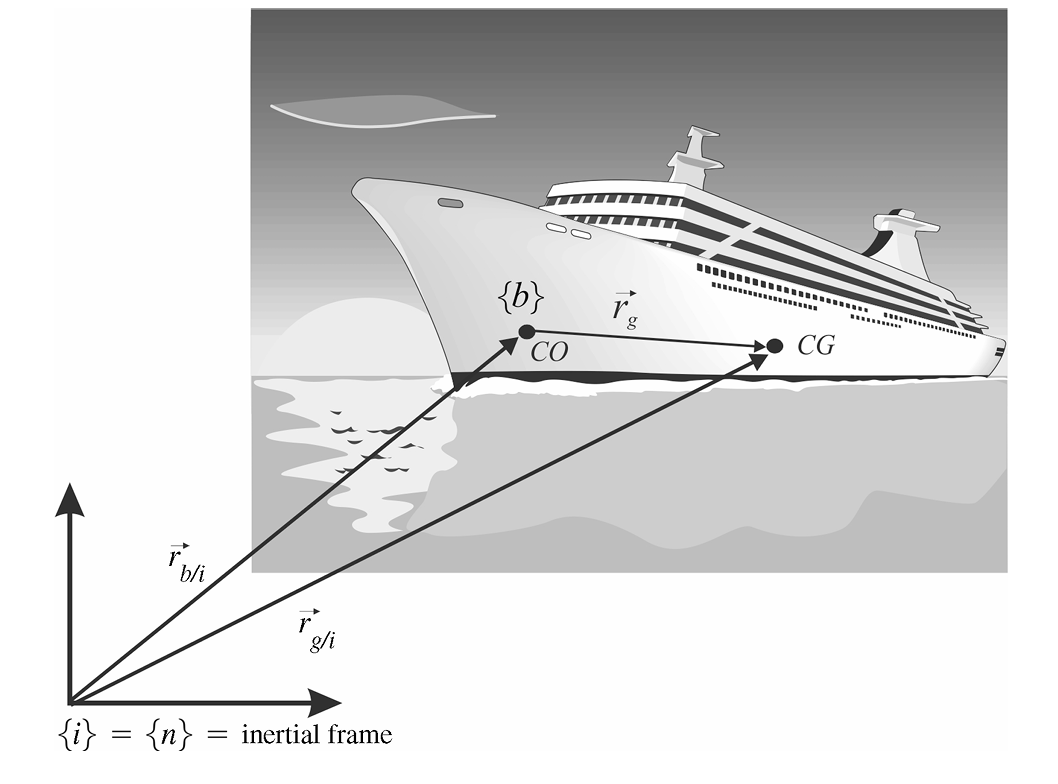
\includegraphics[width=0.5\linewidth]{img/coordinate.png}};
	\end{tikzpicture}
	
	\begin{itemize}
		\item Translational motion
		\item Rotational motion
	\end{itemize}
	
	\vspace{2cm}
	
	\begin{block}{Equations of Motion about CG}
		The Newton-Euler equation could be represented in the matrix form according to
		\begin{align}
			M_{RB}^{CG} \begin{bmatrix}
				\dot{v}_{g/n}^b \\ \dot{\omega}_{b/n}^b
			\end{bmatrix} + C_{RB}^{CG}\begin{bmatrix}
				{v}_{g/n}^b \\ {\omega}_{b/n}^b
			\end{bmatrix} = \begin{bmatrix}
				f_{g}^b \\ m_{g}^b
			\end{bmatrix}
		\end{align}
	\end{block}
\end{frame}

% =========================================
% =========================================

\begin{frame}{6-DOF model of a Rigid Body}
	\framesubtitle{Equations of Motion about CG}
	
	\begin{block}{Translational motion}
		Using Euler's first axiom,
		\begin{align}
			f_g = \dfrac{d}{dt}(mv_{g/i})
		\end{align}
		by several tedious mathematical transformations
		\begin{align}
			m\Big(\dot{v}_{g/n}^b + \omega_{b/n}^b\times v_{g/n}^b\Big) = f_{g}^b
		\end{align}
	\end{block}
	
	
	\begin{block}{Rotational motion}
		Using Euler's second axiom,
		\begin{align}
			m_g = \dfrac{d}{dt}(I_g\omega_{b/i})
		\end{align}
		by several tedious mathematical transformations
		\begin{align}
			I\dot{\omega}_{b/n}^{b} - S(I_g\omega_{b/n}^b) \times \omega_{b/n}^b = m_{g}^b
		\end{align}
	\end{block}
	
	
\end{frame}


% =========================================
% =========================================


\begin{frame}{6-DOF model of a Rigid Body}
	\framesubtitle{Equations of Motion about CO}
	By several SUPER TEDIOUS mathematical transformations
	\begin{block}{Nonlinear 6 DOF Rigid-Body Equations of Motion}
		\begin{align}
			m \big[\dot{u} - vr + wq - x_g(q^2 + r^2) + y_g(pq - \dot{r}) + z_g(pr + \dot{q})\big] = X, \\
			m \big[\dot{v} - wp + ur - y_g(r^2 + p^2) + z_g(qr - \dot{p}) + x_g(qp + \dot{r}) \big] = Y, \\
			m \big[\dot{w} - uq + vp - z_g(p^2 + q^2) + x_g(rp - \dot{q}) + y_g(r \dot{p})\big] = Z,
			\\
			I_x \dot{p} + (I_z - I_y)qr - (r + pq)I_{xz} + (r^2 - q^2)I_{yz} + (pr - \dot{q})I_{xy} & \notag\\
			+ m \big[ y_g(\dot{w} - uq + vp) - z_g(\dot{v} - wp + ur) )= K, \\
			I_y \dot{q} + (I_x - I_z)rp - (p + qr)I_{xy} + (p^2 - r^2)I_{zx} + (qp - \dot{r})I_{yz} & \notag \\
			+ m \big[ z_g(\dot{u} - vr + wq) - x_g(\dot{w} - uq + vp) ) = M, \\
			I_z \dot{r} + (I_y - I_x)pq - (q + rp)I_{xz} + (q^2 - p^2)I_{xx} + (rq - \dot{p})I_{zx} & \notag \\
			+ m \big[ x_g(\dot{v} - wp + ur) - y_g(\dot{u} - vr + wq)) = N.
		\end{align}
	\end{block}
\end{frame}

% =========================================
% =========================================



\begin{frame}{6-DOF model of a Rigid Body}
	\framesubtitle{Matrix Form}
	\begin{block}{Rigid-body dynamics model}
		\begin{align}
			M_{RB}\dot{\nu} + C_{RB}\nu = \tau_{RB}
		\end{align}
		where
		\begin{align}
			M_{RB} = \begin{bmatrix}
				mI_{3\times 3} & -mS(r_g^b) \\
				mS(r_g^b) & I_b
			\end{bmatrix} \\
			C_{RB} = \begin{bmatrix}
				0_{3\times 3} & -S(M_{11}\nu_1 + M_{12}\nu_2) \\
				-S(M_{11}\nu_1 + M_{12}\nu_2) & -S(M_{21}\nu_1 + M_{22}\nu_2)
			\end{bmatrix} 
		\end{align}
	\end{block}
\end{frame}



% =========================================
% =========================================




\begin{frame}{6-DOF model of a Rigid Body}
	\framesubtitle{Linearized 6 DOF Rigid body Equation of Motion}
	
	
\end{frame}
% =========================================
% =========================================




\begin{frame}{Dynamics model}
	\framesubtitle{Simplifyed 6 DOF Rigid body Equation of Motion}
	\begin{itemize}
		\item The Origin CO coincides with the CG
		\item Translation of the origin CO such that $I_b$ becomes diagonal
	\end{itemize}
	\begin{block}{Simplifyed 6 DOF Rigid body Equation of Motion}
		\begin{align}
			m \big[ \dot{u} - vr + wq - x_g (q^2 + r^2) + y_g (pq - \dot{r}) + z_g (pr + \dot{q}) \big] &= X, \\
			m \big[ \dot{v} - wp + ur - y_g (r^2 + p^2) + z_g (qr - \dot{p}) + x_g (qp + \dot{r}) \big] &= Y, \\
			m \big[ \dot{w} - uq + vp - z_g (p^2 + q^2) + x_g (rp - \dot{q}) + y_g (rq + \dot{p}) \big] &= Z, \\
			I_x \dot{p} + (I_z - I_y) qr + m \big[ y_g (\dot{w} - uq + vp) - z_g (\dot{v} - wp + ur) \big] &= K, \\
			I_y \dot{q} + (I_x - I_z) rp + m \big[ z_g (\dot{u} - vr + wq) - x_g (\dot{w} - uq + vp) \big] &= M, \\
			I_z \dot{r} + (I_y - I_x) pq + m \big[ x_g (\dot{v} - wp + ur) - y_g (\dot{u} - vr + wq) \big] &= N.
		\end{align}
	\end{block}
\end{frame}


% =========================================
% =========================================
